\begin{figure}[h!]
  \centering
  \begin{tikzpicture}
    [spy scope= {circle, magnification=6, size=3cm},
      every spy on node/.style={draw, Red, thick},
      every node/.style={inner sep=0},
      label distance=-1cm]

    \node (original) {
      \begin{minipage}{0.45\textwidth}
        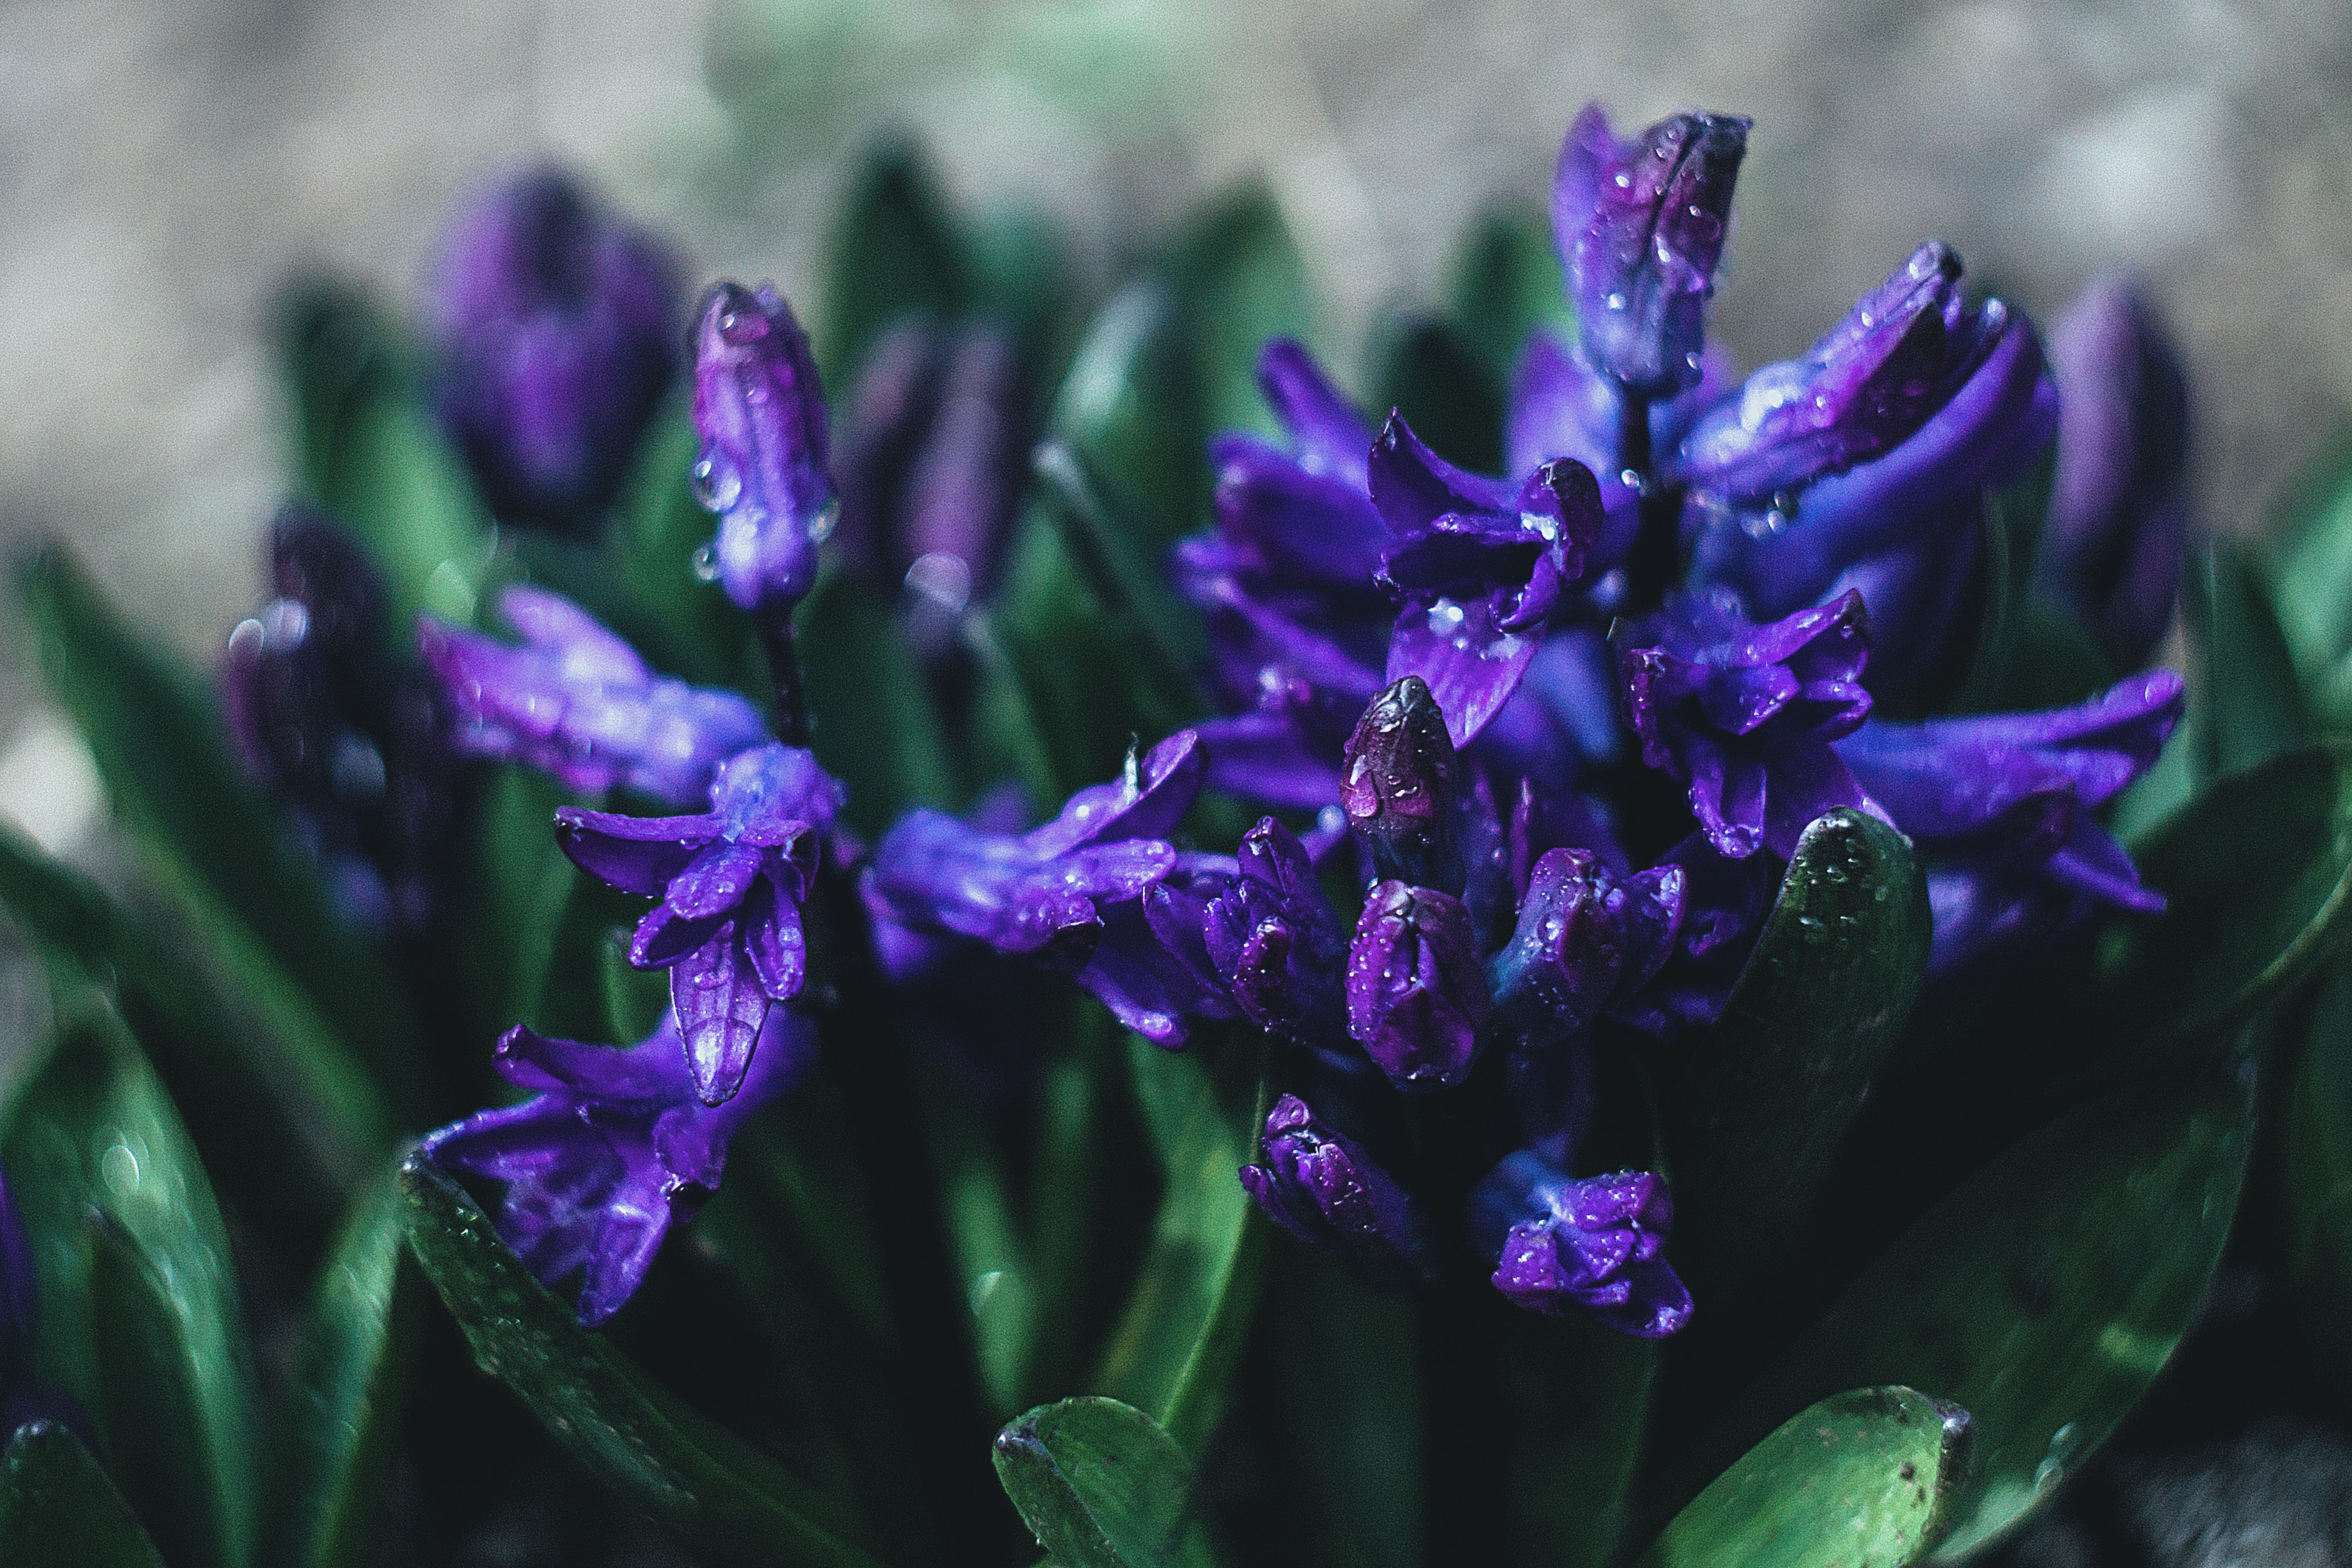
\includegraphics[width=1\textwidth]{flowers/flowers.png}
        \caption*{Original}
      \end{minipage}
    };
    \node [right= of original] (10mb) {
      \begin{minipage}{0.45\textwidth}
        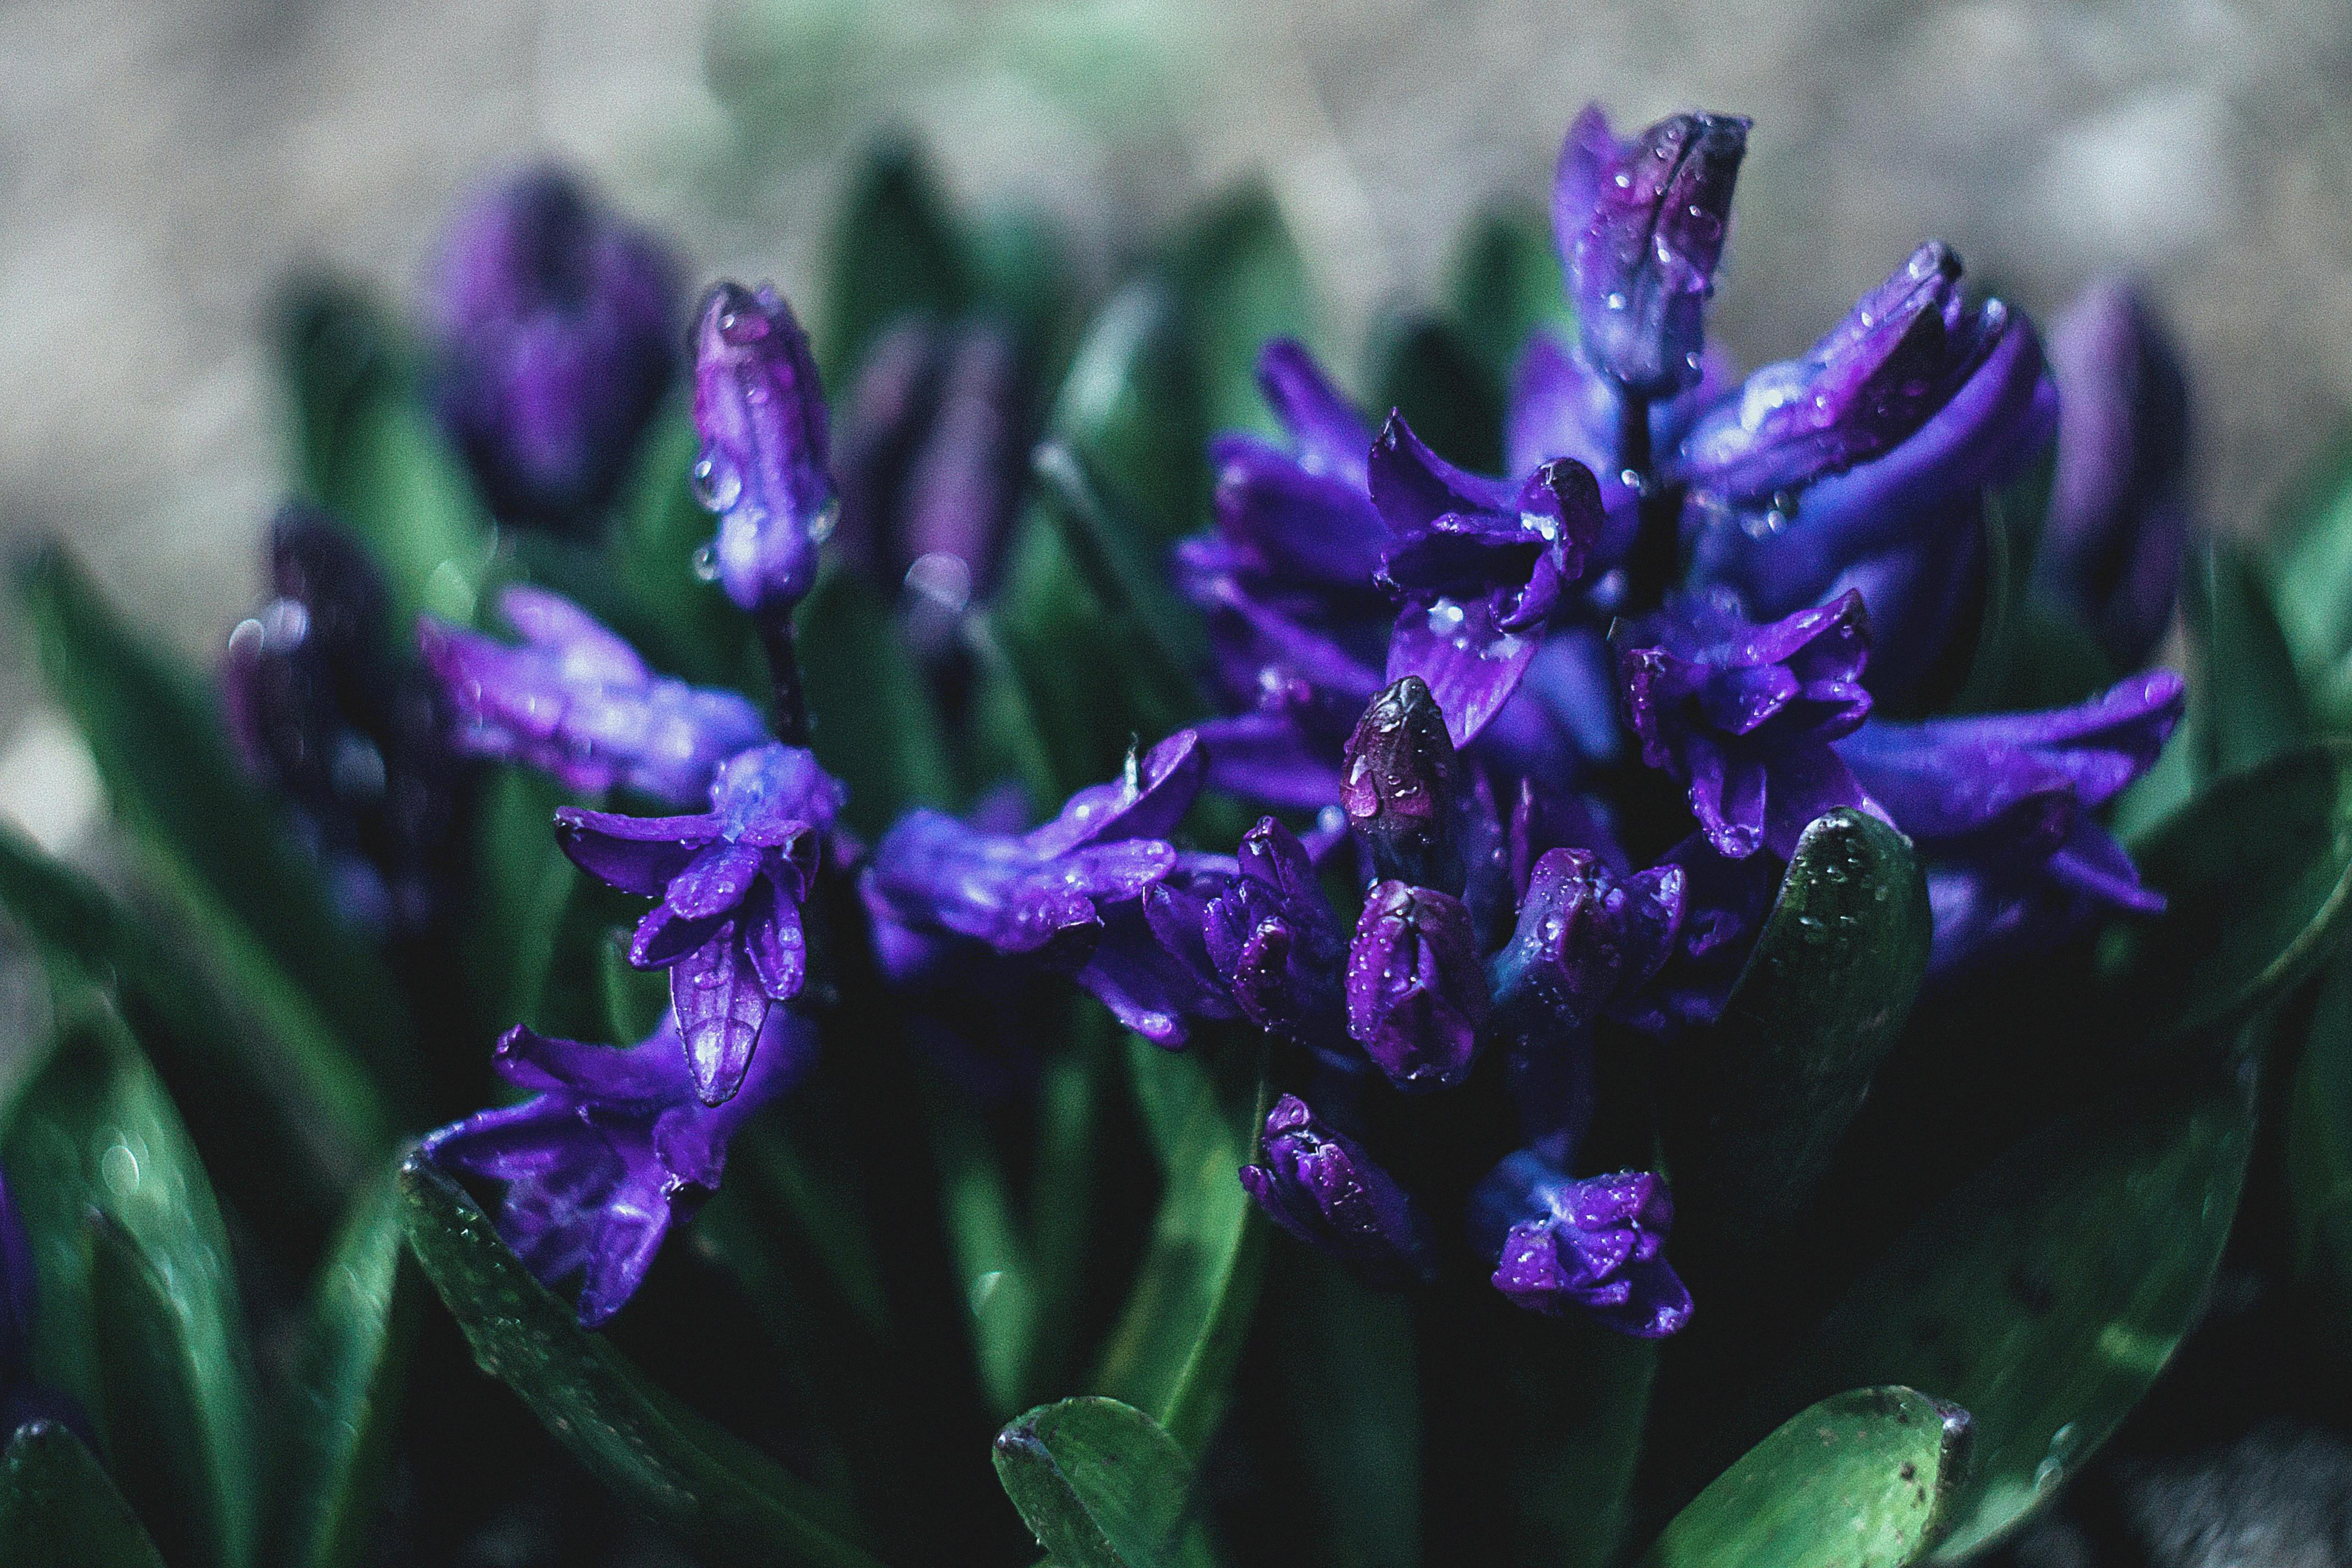
\includegraphics[width=1\textwidth]{flowers/flowers-48.png}
        \caption*{48\,\% (\num{17.5}\,MB)}
      \end{minipage}
    };
    \node [below=0.5cm of original] (20mb) {
      \begin{minipage}{0.45\textwidth}
        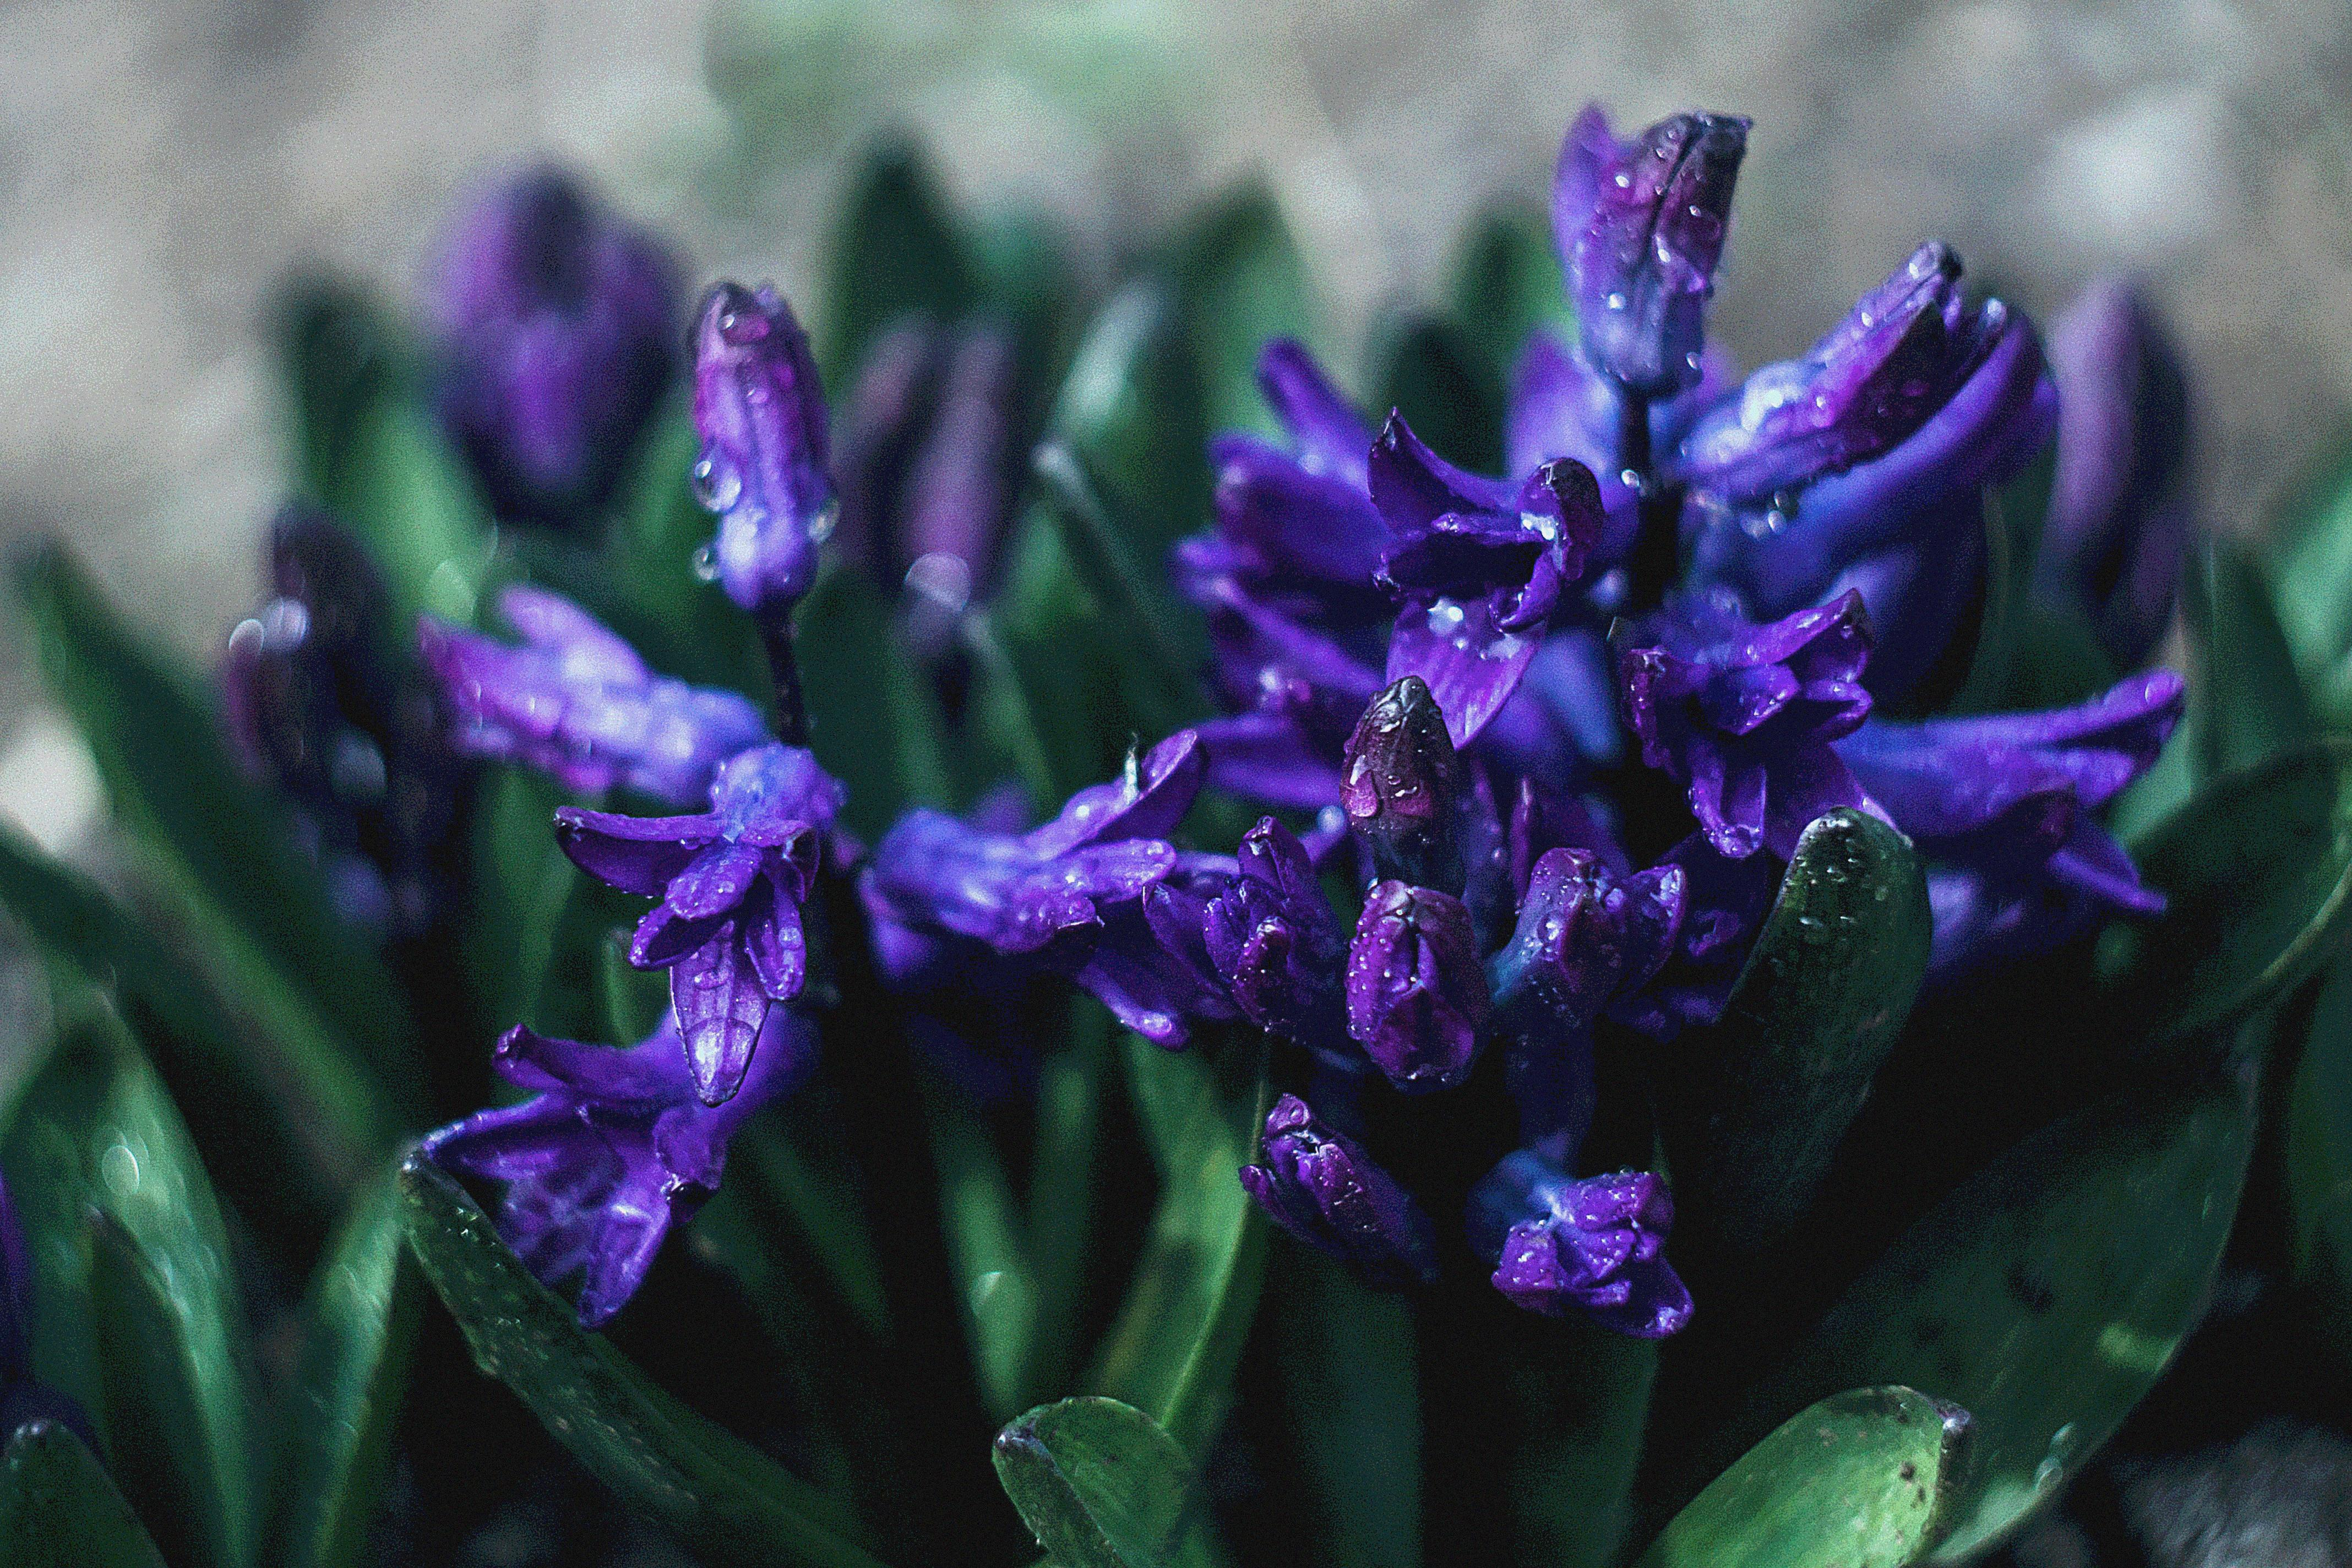
\includegraphics[width=1\textwidth]{flowers/flowers-60.png}
        \caption*{60\,\% (\num{21.9}\,MB)}
      \end{minipage}
    };
    \node [below=0.5cm of 10mb] (30mb) {
      \begin{minipage}{0.45\textwidth}
        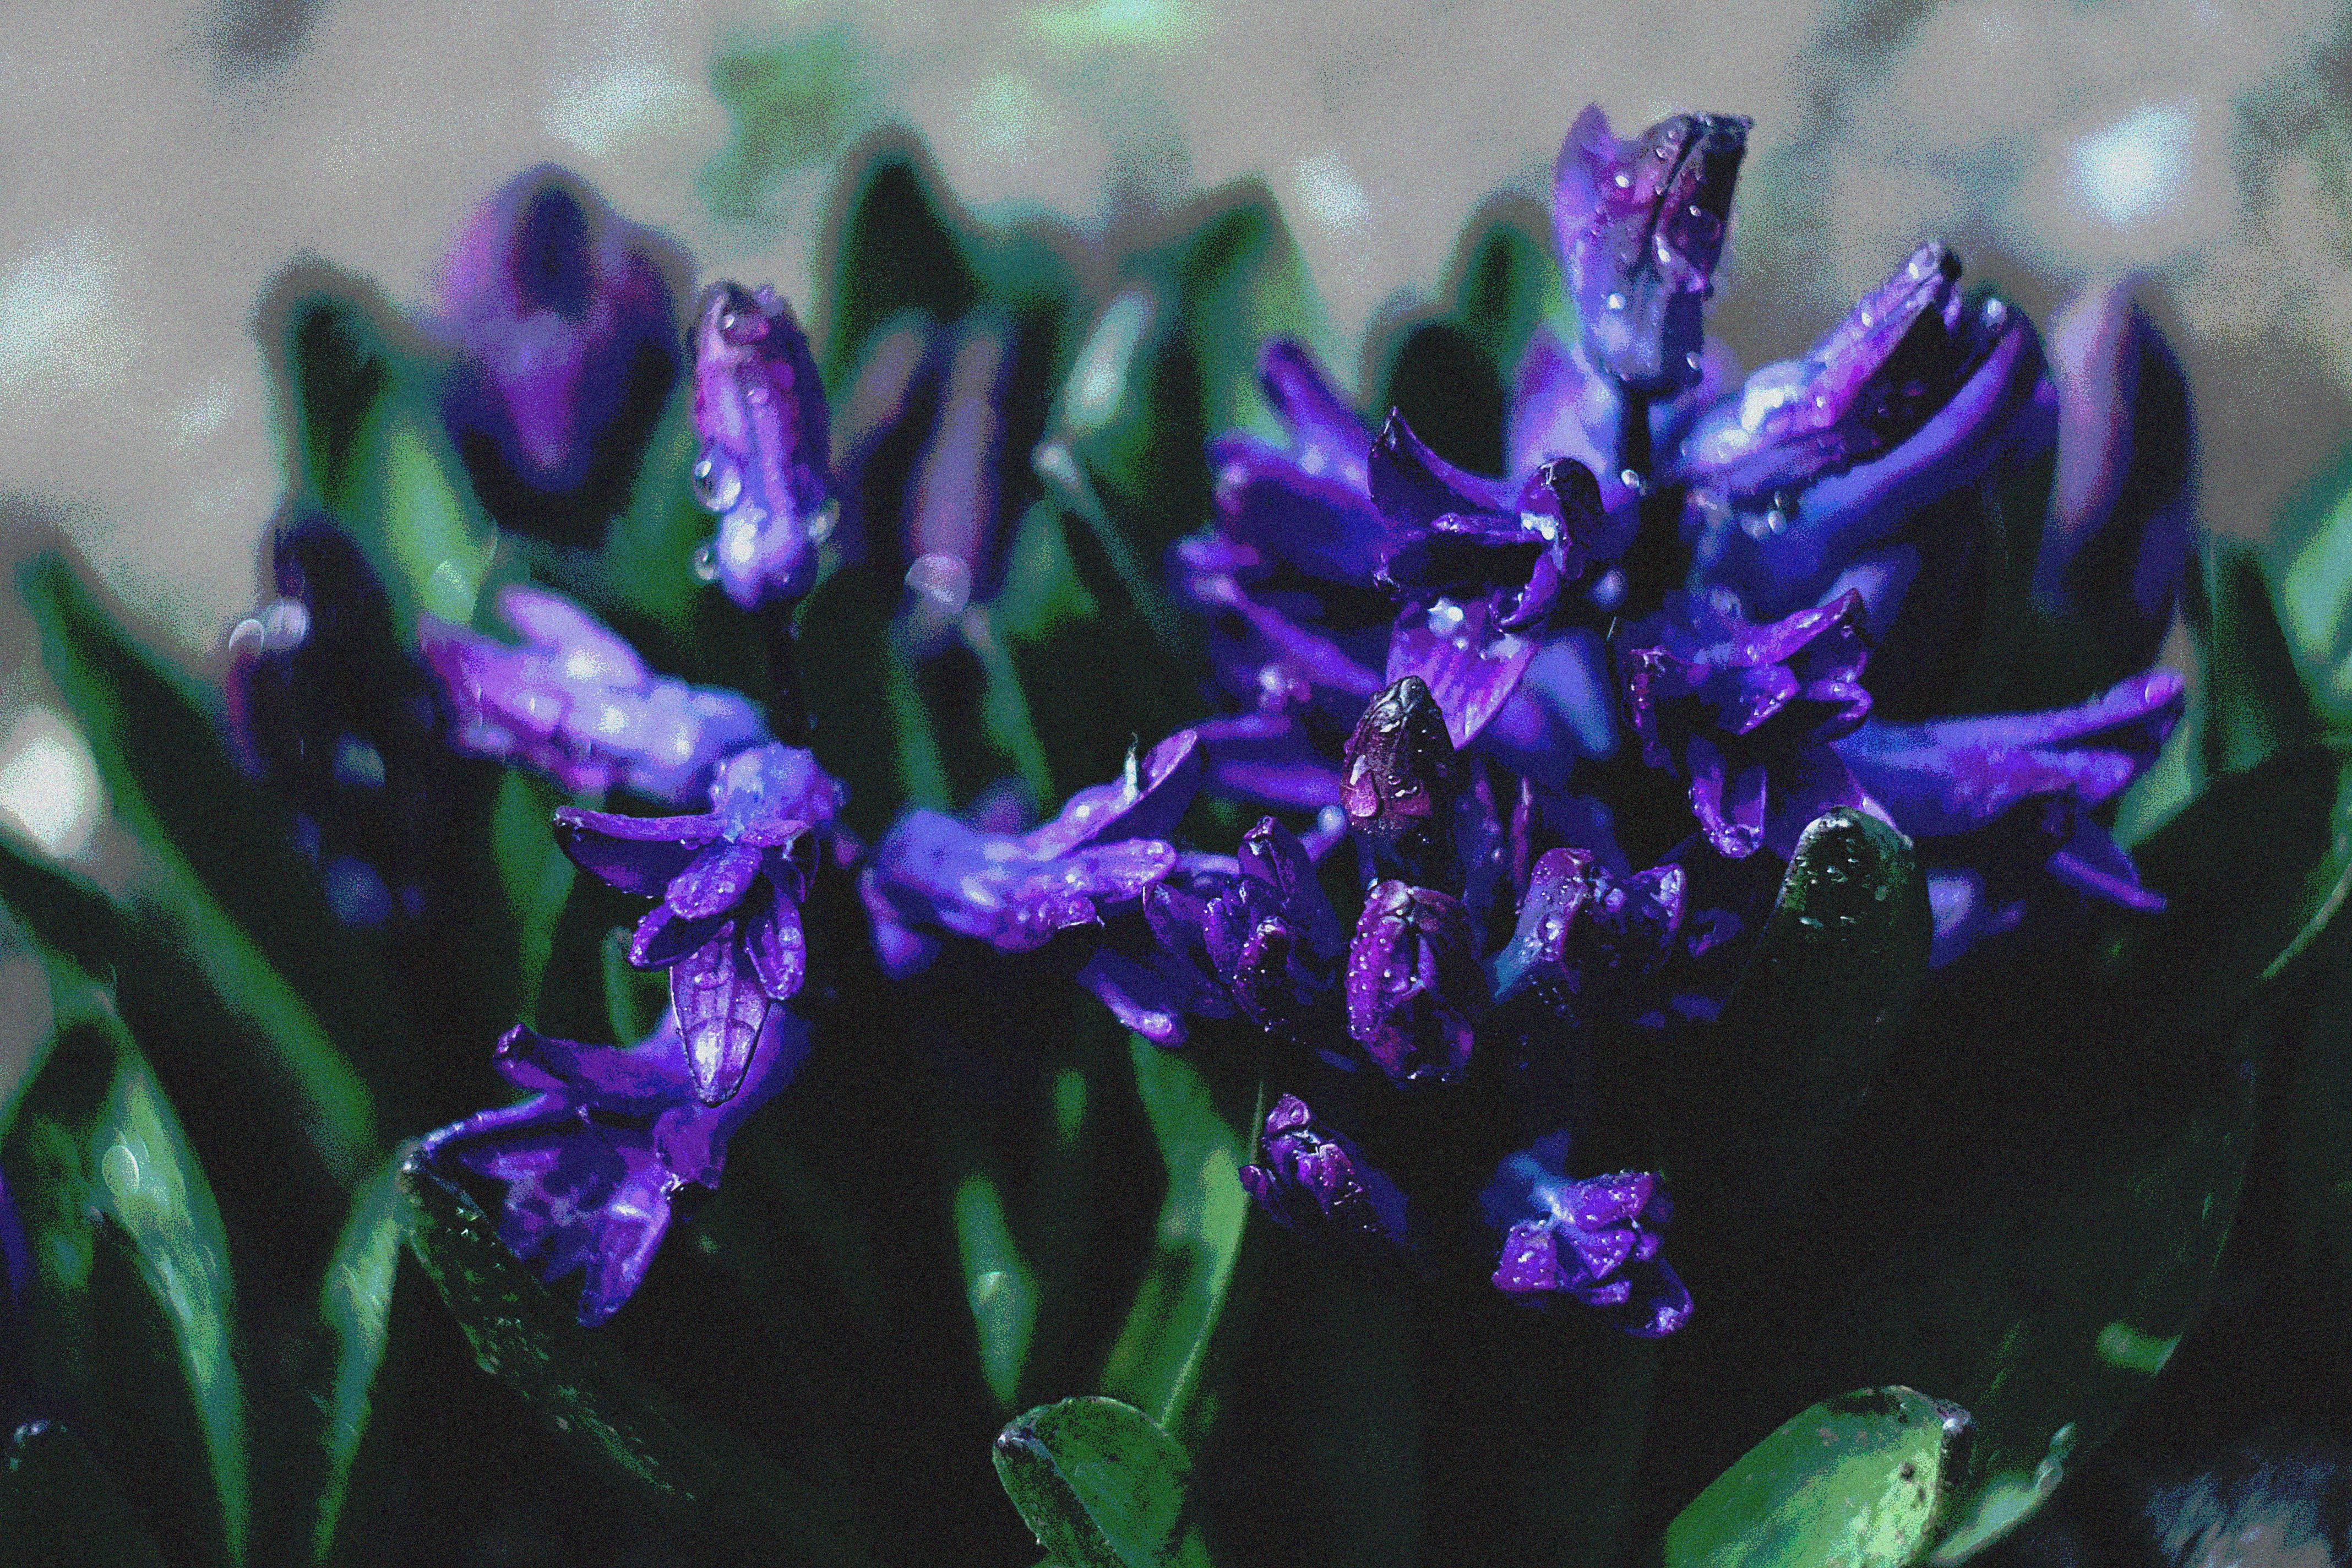
\includegraphics[width=1\textwidth]{flowers/flowers-72.png}
        \caption*{72\,\% (\num{26.3}\,MB)}
      \end{minipage}
    };

    \matrix [column sep=3.5cm] at ($(original.north)!0.5!(10mb.north) + (0,3.5cm)$) {
      \coordinate (a); & \coordinate (b); & \coordinate (c); & \coordinate (d); \\
    };

    \coordinate (spy-on) at (1.05cm,-0.55cm);

    \spy on ($(original.north) + (spy-on)$) in node[label=below:Original] at (a);
    \spy on ($(10mb.north) + (spy-on)$) in node[label=below:48\,\%] at (b);
    \spy on ($(20mb.north) + (spy-on)$) in node[label=below:60\,\%] at (c);
    \spy on ($(30mb.north) + (spy-on)$) in node[label=below:72\,\%] at (d);

  \end{tikzpicture}
  \caption{Blumen mit einer Größe von 2848 $\times$ 4272 Pixel.
    Gute Bildqualität bis zu 22\,MB versteckter
    Nachricht ($\bmax \approx \num{36.5}$\,MB).}
  \label{fig:example-flowers}
\end{figure}
